\documentclass{standalone}
\usepackage{tikz}
\usetikzlibrary {arrows.meta, automata,positioning}
\usetikzlibrary{angles, quotes}
\usepackage{pgfplots}
\pgfplotsset{compat=1.18}




% ref:
% https://tex.stackexchange.com/questions/118563/moebius-strip-using-tikz
% https://tex.stackexchange.com/questions/590735/angle-between-two-vectors-tikz-latex
\tikzset{
    >={Latex}
}


\begin{document}
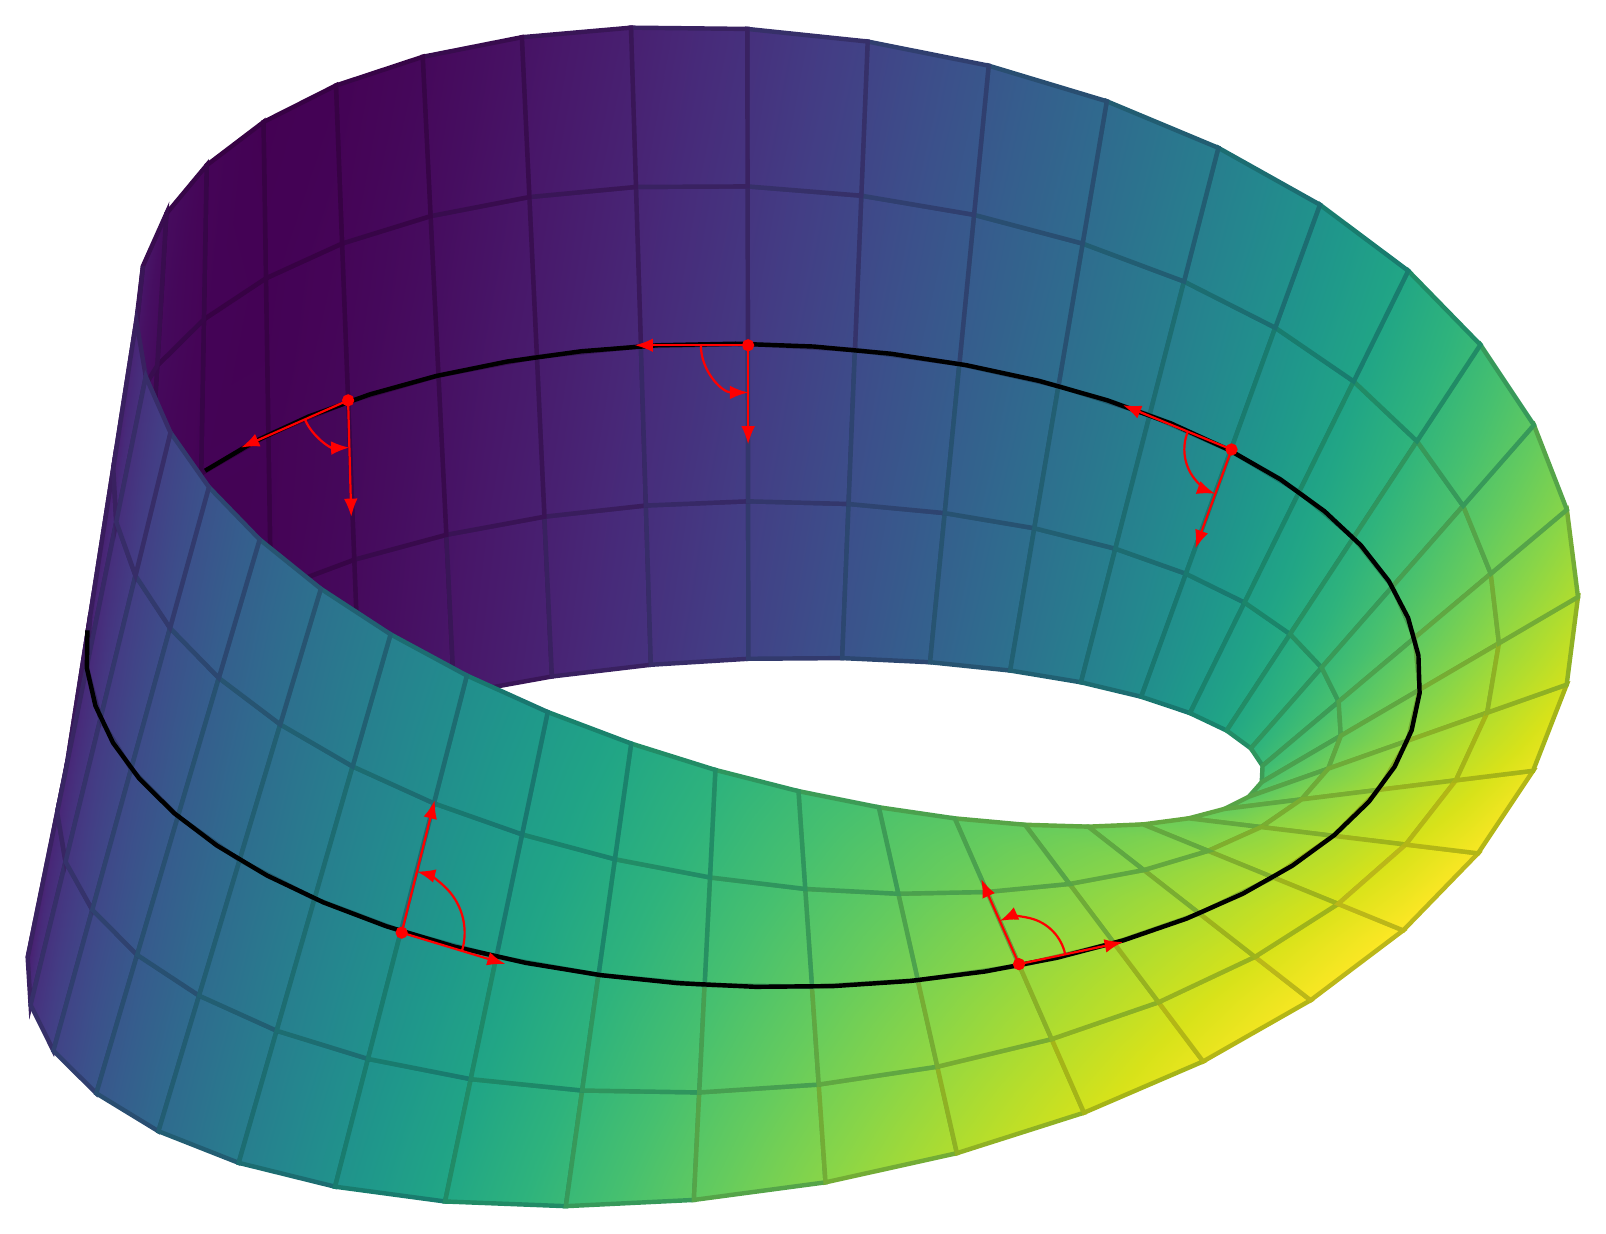
\begin{tikzpicture}[scale=4, every edge quotes/.append style = {auto, sloped}]
\begin{axis}[
    hide axis,
    view={40}{45}
]
% \addplot3 [
%     surf, shader=faceted interp,
%     point meta=x,
%     colormap/blackwhite,
%     samples=40,
%     samples y=10,
%     z buffer=sort,
%     domain=0:360,
%     y domain=-0.5:0.5
% ] (
%     {(2*cos(x)+0.5*y*cos(x/2)))*cos(x)},
%     {(2*sin(x)+0.5*y*cos(x/2)))*sin(x)},
%     {0.5*y*sin(x/2)}
% );
\addplot3 [
    surf, shader=faceted interp,
    point meta=x,
    colormap/viridis,
    samples=40,
    samples y=5,
    z buffer=sort,
    domain=0:360,
    y domain=-0.5:0.5
] (
    {(1+0.5*y*cos(x/2)))*cos(x)},
    {(1+0.5*y*cos(x/2)))*sin(x)},
    {0.5*y*sin(x/2)}
);

\addplot3 [
    samples=50,
    domain=-145:184,
    samples y=0
] (
    {cos(x)},
    {sin(x)},
    {0});
\end{axis}

% test node
\filldraw[red] (2.11, 2.08) circle (.5pt);
\filldraw[red] (4.07, 1.98) circle (.5pt);
\filldraw[red] (1.94, 3.77) circle (.5pt);
\filldraw[red] (3.21, 3.945) circle (.5pt);
\filldraw[red] (4.745, 3.614) circle (.5pt);


% draw arrow
% 1.
\begin{scope}
    \draw[->, red, thick] (2.11, 2.08) coordinate (O)  -- (2.215, 2.5) coordinate (f1);
    \draw[->, red, thick] (2.11, 2.08) -- (2.44, 1.98) coordinate (f2);
    \pic [thick, draw, red, ->, angle radius = 8mm, angle eccentricity=0, ""] {angle = f2--O--f1};    
\end{scope}
% 2.
\begin{scope}
    \draw[->, red, thick] (4.07, 1.98) coordinate (O)  -- (3.95, 2.25) coordinate (f1);
    \draw[->, red, thick] (4.07, 1.98) -- (4.4, 2.05) coordinate (f2);
    \pic [thick, draw, red, ->, angle radius = 6mm, angle eccentricity=0, ""] {angle = f2--O--f1};    
\end{scope}
% 3.
\begin{scope}
    \draw[->, red, thick] (1.94, 3.77) coordinate (O)  -- (1.95, 3.4) coordinate (f1);
    \draw[->, red, thick] (1.94, 3.77) -- (1.6, 3.62) coordinate (f2);
    \pic [thick, draw, red, ->, angle radius = 6mm, angle eccentricity=0, ""] {angle = f2--O--f1};    
\end{scope}
% 4.
\begin{scope}
    \draw[->, red, thick] (3.21, 3.945) coordinate (O)  -- (2.85, 3.945) coordinate (f1);
    \draw[->, red, thick] (3.21, 3.945) -- (3.21, 3.63) coordinate (f2);
    \pic [thick, draw, red, ->, angle radius = 6mm, angle eccentricity=0, ""] {angle = f1--O--f2};    
\end{scope}
% 5.
\begin{scope}
    \draw[->, red, thick] (4.745, 3.614) coordinate (O)  -- (4.4, 3.755) coordinate (f1);
    \draw[->, red, thick] (4.745, 3.614) -- (4.63, 3.3) coordinate (f2);
    \pic [thick, draw, red, ->, angle radius = 6mm, angle eccentricity=0, ""] {angle = f1--O--f2};    
\end{scope}

\end{tikzpicture}

\end{document}